\section{Theoretical Background}
\label{sec:theoretical_background}

\subsection{Machine Learning}
\subsubsection{Types of Machine Learning}
\subsubsection{Classification}

\subsection{Building Blocks of Neural Networks}

\subsubsection{Fully Connected Layer}
\subsubsection{Convolutional Layers}
\subsubsection{Pooling Layers}
\subsubsection{Batch Normalization Layers?}
\subsubsection{Softmax Loss Function}

\subsection{Recurrent Neural Networks}
\subsubsection{Long Short Term Memory Networks}

\subsection{Hybrid Networks}
\label{sec:hybrid_networks}

	\begin{figure}[]
  		\centering
    	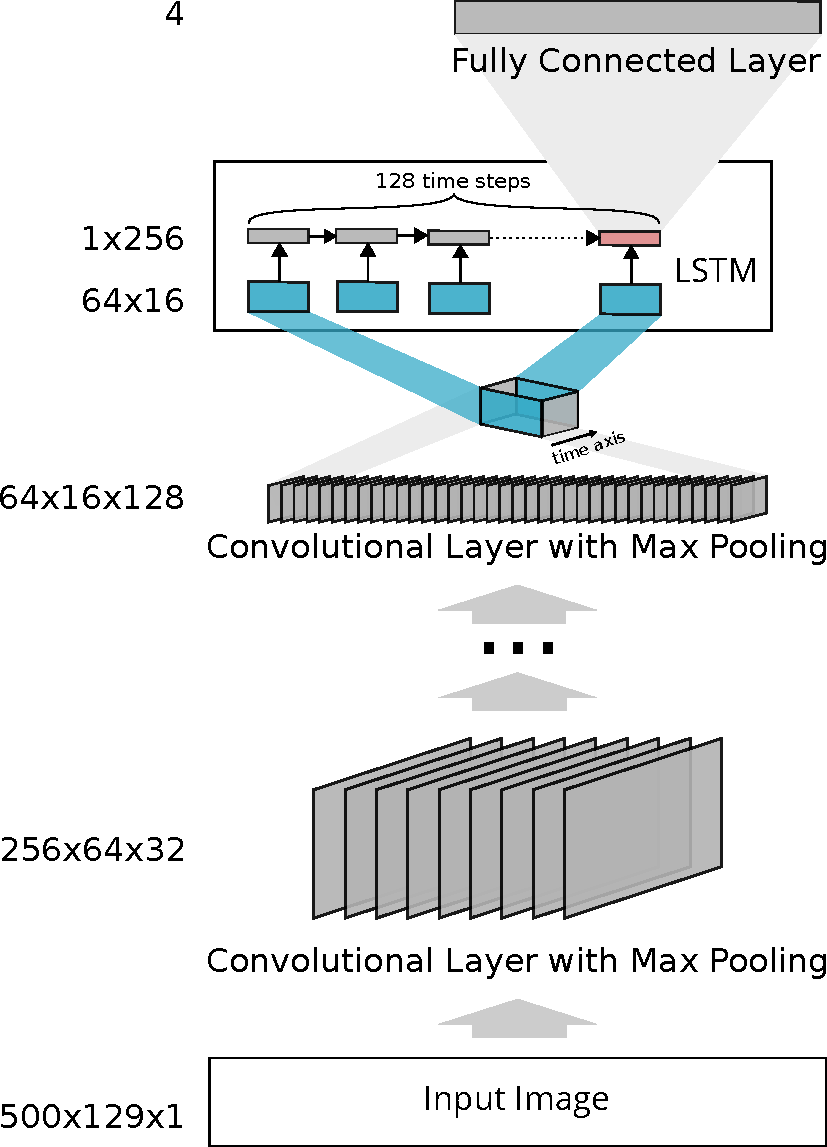
\includegraphics[width=\textwidth, keepaspectratio]{img/crnn.pdf}
    	\caption{Our proposed CRNN hybrid network architecture consists of two networks. A CNN transforms our input images into an intermediary representation of our audio frequencies. The 3D output of final convolutional layer of the CNN is sliced along the x-axis (time axis) into 2D time steps still containing all feature map information. The output of the final LSTM time step is fed into a fully connected layer for classification.}
    	\label{fig:crnn}
	\end{figure}
	
	\begin{figure}[]
  		\centering
    	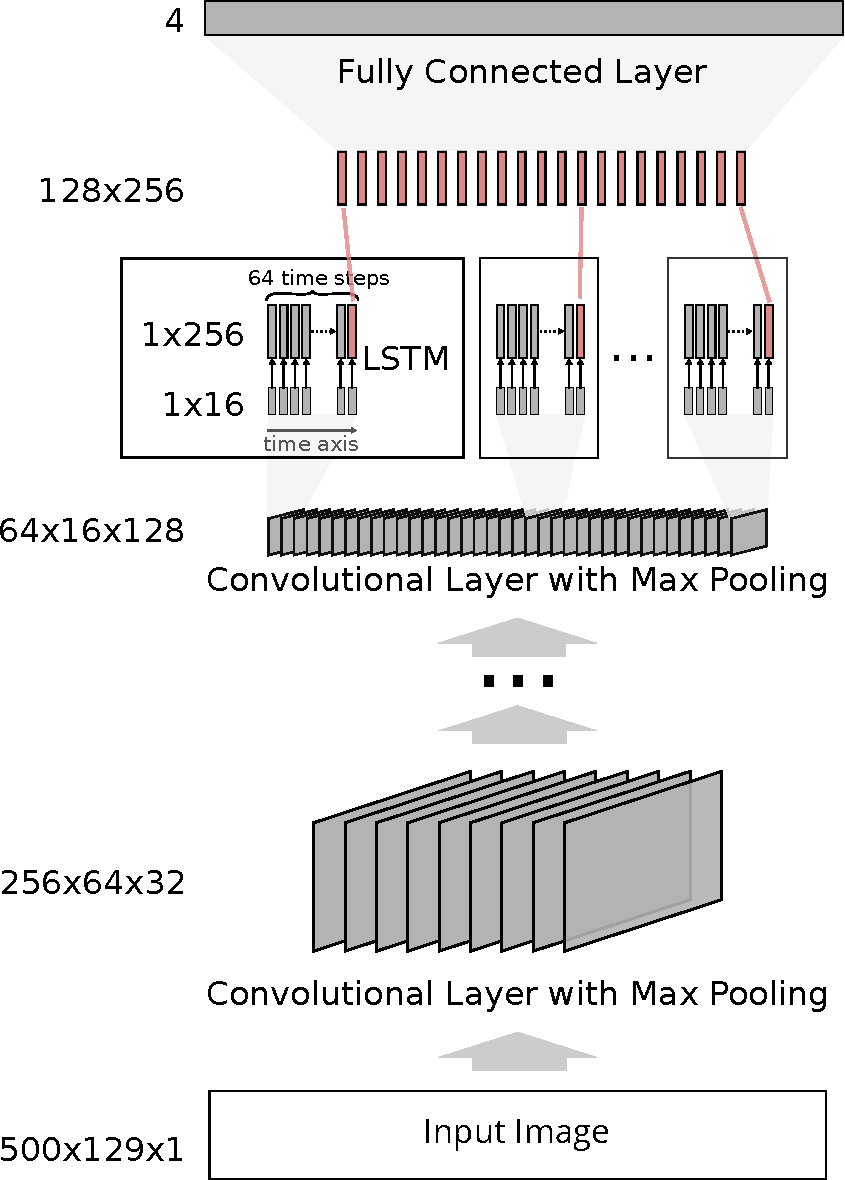
\includegraphics[width=\textwidth, keepaspectratio]{img/crnn2.pdf}
    	\caption{An alternative approach for a hybrid CRNN network. Each single feature map of the final convolutional layer is fed to separate LSTM networks as a 2D input. Each LSTM interprets the vector entries along the x-axis as time steps and operates on thin slice of the data. The output of the final time step of each LSTM is concatenated into a single vector serving as the input to a fully connected classification layer.}
    	\label{fig:crnn}
	\end{figure}

    \begin{itemize}
        \item Convolutional Recurrent Neural Networks
        \item What is their purpose? Averaging over predictions / fusion
    \end{itemize}

\subsection{Audio Representations}
\label{sec:audio_representations}
    \begin{itemize}
        \item MFCC
        \item Spectrogram
        \item Waveform
        \item Mel-scale
        \item frequency --> phoneme --> word --> sentence --> language
    \end{itemize}